
\section{\nmu Algorítimos de \textit{string matching} exatos} % (fold)
\label{sec:algor_timos_de_string_matching_exatos}

Para a busca com algorítimos de \textit{string matching} exatos, foram considerado três métodos distintos:

\begin{description}
	\item[Expressão Regular:] Método atual de como a verificação é realizada atualmente. Foi previamente comentado na sessão de \nameref{sec:algoritimos_de_textit}.
	\item[Knuth-Morris-Pratt:] Método que faz de uso do conceito de autômatos de estados para agilizar a busca. Previamente apresentado na sessão \ref{ssub:knuth_morris_pratt_}.
	\item[Rabin-Karp:]  Método que faz de uso de \textit{hash}. Foi previamente comentado na sessão \ref{ssub:rabin_karp}.
\end{description}

Após a coleta de $150$ chamadas de cada pacote usando os algorítimos apontados acima, a \autoref{ssub:rabin_karp} foi criada contendo a mediana dos tempos de execução de cada método para os pacotes selecionados.

\begin{figure}[htbp]
  \centering
  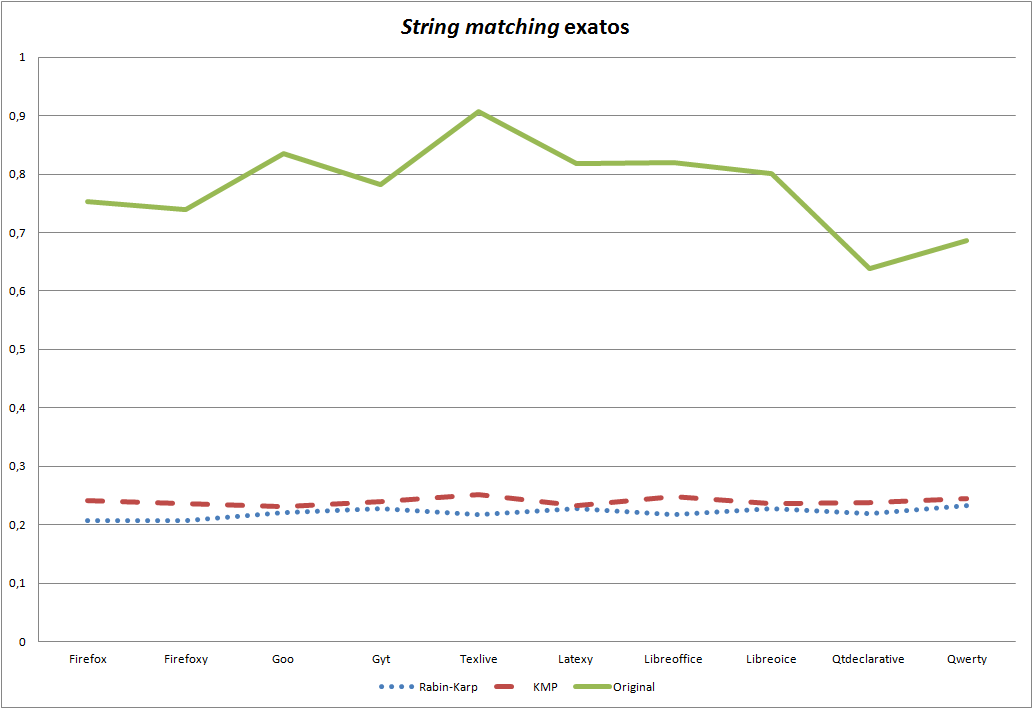
\includegraphics[width=0.95\textwidth]{figuras/tempo-rk_kmp_std}
  \caption{Estimativa de tempo para pacotes usando algorítimos de busca exata}
  \label{tempo_rk_kmp_std}
\end{figure}

Como podemos observar, tanto o \textit{Rabin-Karp} quanto o \textit{KMP} tiveram um rendimento de cerca de $\frac{1}{3}$ do tempo gasto atualmente com o uso de expressões regulares, sendo no tempo geral, o método de \textit{Rabin-Karp} possui um desempenho ligeiramente melhor.


\begin{figure}[htbp]
  \centering
  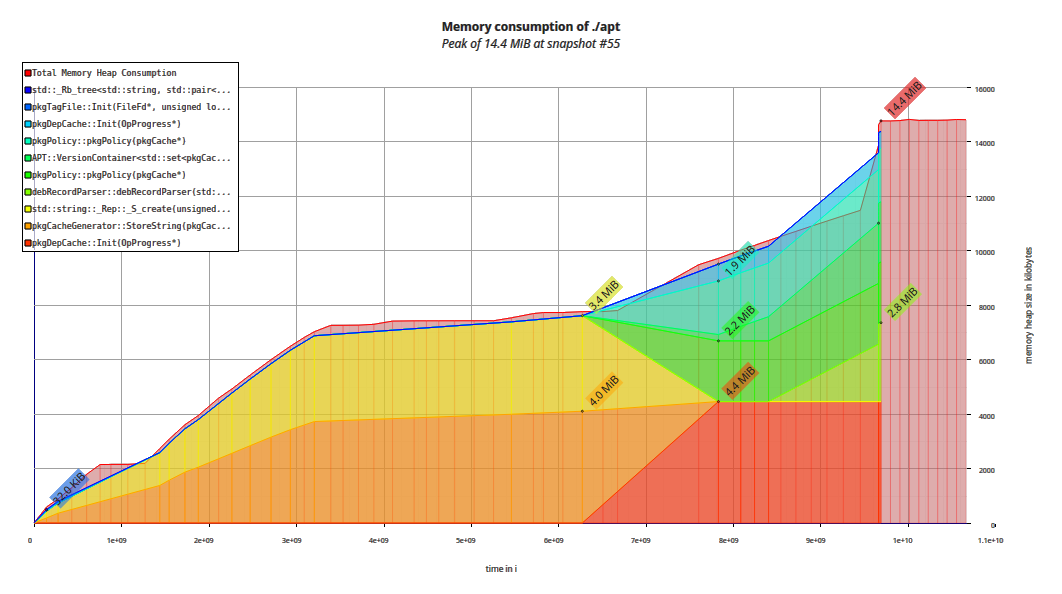
\includegraphics[width=0.95\textwidth]{figuras/memory_rk.png}
  \caption{Apontamento de uso de memória com uso do método de \textit{Rabin-Karp}}
  \label{memory_rk}
\end{figure}

O consumo total de memória para ambos os métodos, \textit{Rabin-Karp} na \autoref{memory_rk} e expressões regulares na \autoref{memory_std},  apresentaram resultados similares, porém o método de \textit{Rabin-Karp} faz um uso de memória mais pontual, alcançando o pico de consumo ao final do processo, quando esta prestes a liberar os recursos. Já o método de expressões regulares apresenta um consumo mais linear de memória. 


\begin{figure}[htbp]
  \centering
  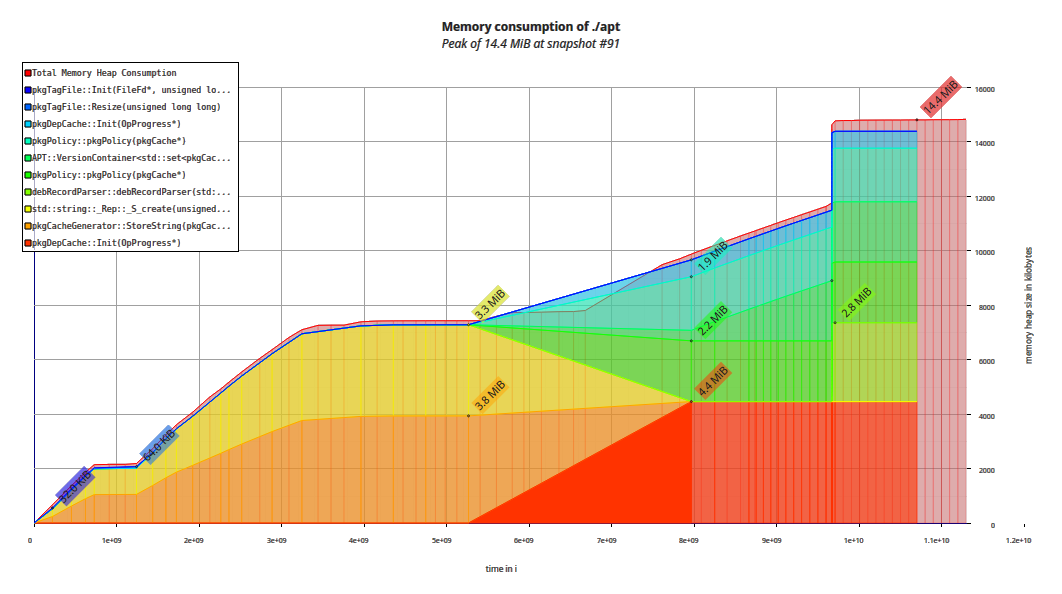
\includegraphics[width=0.95\textwidth]{figuras/memory_regex.png}
  \caption{Apontamento de uso de memória com uso de expressões regulares}
  \label{memory_std}
\end{figure}

Um gasto mais prologado de memória vem a ser prejudicial para sistemas em que diversos processos possam estar sendo executados em conjunto, todavia o grau de consumo é muito baixo para o posicionamento de que o consumo por um período mais extenso venha a ser prejudicial, visto que para um sistema com $2GB$ de memória RAM, $15MB$ seria um valor irrisório de menos de $1\%$ do total de recurso disponível.
% chapter analise_de_resultados (end)

